\documentclass{article}
\usepackage[utf8]{inputenc}
\usepackage{datetime}
\usepackage{enumerate}
\usepackage{textcomp}
\usepackage{amsmath}
\usepackage{tikz}
\usetikzlibrary{arrows}
\usepackage{graphicx}
\graphicspath{ {./images/} }

\title{\bf \Large ASSIGNMENT 2}
\author{Xinhao Luo}
\date{\today}

\def\math#1{$#1$}

\setlength{\textheight}{8.5in}
\setlength{\textwidth}{6.5in}
\setlength{\oddsidemargin}{0in}
\setlength{\evensidemargin}{0in}
\voffset0.0in

\begin{document}
\maketitle
\medskip

\section{Exercise 1.8}
\math{v \leq 0.1} means there will be either 1 or 0 red marble in our samples, so we have:

\begin{itemize}
    \item [1 marble] \math{{10 \choose 1} * 0.9^1 * 0.1^{10 - 1} = 9 \times 10^{-1}}
    \item [0 marble] \math{{10 \choose 0} * 0.9^0 * 0.1^{10} = 1 \times 10^{-10}}
\end{itemize}

\math{9 \times 10^{-9} + 10^{-10} = 9.1 \times 10^{-9}}

\section{Exercise 1.9}

Here we have \math{\epsilon = 0.9 - 0.1 = 0.8}, so \math{P[\lvert \upsilon - \mu \rvert > \epsilon] \leq 2e^{-2\epsilon^2N} = 2 * e^{-2 * 0.8^2 * 10} = 5.52 \times 10^{-6}}

The Hoeffding Bound is greater than the result in 1.8

\section{Exercise 1.10}

\begin{enumerate}[a)]
    \item All \math{\mu} should be 0.5
    \item 
        \begin{itemize}
            \item [\math{V_1}] 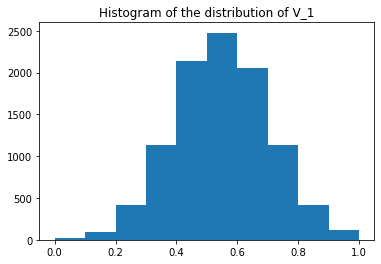
\includegraphics{1.10/2}
            \item [\math{V_{rand}}] 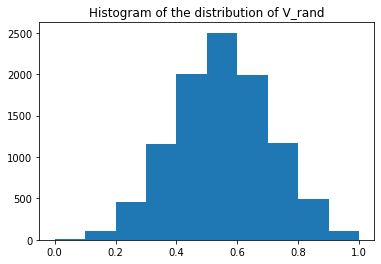
\includegraphics{1.10/1}
            \item [\math{V_{min}}] 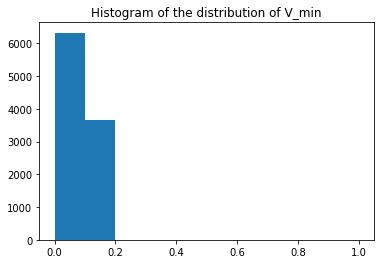
\includegraphics{1.10/3}
        \end{itemize}
    \item 
        \begin{itemize}
            \item [\math{V_1}] 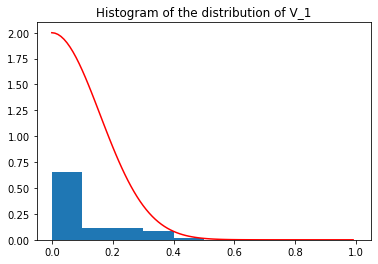
\includegraphics{1.10/5}
            \item [\math{V_{rand}}] 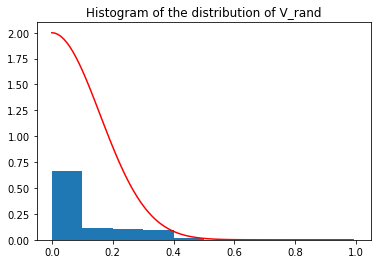
\includegraphics{1.10/4}
            \item [\math{V_{min}}] 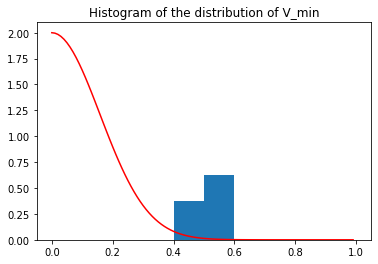
\includegraphics{1.10/6}
        \end{itemize}
    \item \math{c_1} and \math{c_{rand}} obey the Hoeffding bound while the \math{c_{min}} disobey. \math{c_1} and \math{c_{rand}} are random picking and they have the same pattern. \math{c_{min}} has changed selection after the sampling and break the Hoeffding Inequality.
    \item Here let's say we have 1000 bins and each bin has equal number of red and white balls. For each bin we pick 10 balls and calculate \math{\upsilon}. For \math{c_1}, it means we only take results from first bin, and \math{c_{rand}} is to pick a random bin. These results will obey the Hoeffding bound. However, \math{c_{min}} will follow the bin has lower frequency, which is a not fixed hypothesis(changed on every coin flip), though it is closely related to the set.
\end{enumerate}

\section{Exercise 1.11}
\begin{enumerate}[a)]
    \item Can't guaranteed. We have no idea about the outside. E.g. If we have \math{p < 0.5} but for the data \math{D} we have all \math{+1}. We will choose hypothesis that always get \math{+1} which definitely not better than random.
    \item Yes, it is possible. As the same setting in a), \math{C} will choose \math{-1} which is better than what \math{S} has chosen.
    \item With \math{p > 0.9}, \math{S} is better than \math{C} if there are more than 13 \math{+1} in the \math{D}, which will make \math{C} choose \math{-1}. Here we have the probability: 
    \begin{equation}
        \begin{split}
            P = \sum^{25}_{x = 13}{25 \choose x}0.9^x * 0.1^{25 - x} = \frac{624999898697864988370959}{625000000000000000000000} \approx 0.9999998
        \end{split}
    \end{equation}
    \item No, as \math{S} will always choose from the hypothesis based on \math{D}, where \math{D} is an approximation of the outside, \math{S} will always make the better decision and \math{C} will have to choose the imperfect one. Even when \math{p = 0.5}, \math{C} cannot be better than \math{S}.
\end{enumerate}

\section{Exercise 1.12}

C, since it is not possible to guarantee to find a \math{g} that \math{E_{out}(g) \approx E_{in}(g)} with the data points provided here. Even though we may find a \math{E{in} \approx 0}, but at the same time we can't keep \math{E_{out}(g) \approx E_{in}(g)}. C is the best matched statement among the three.

\section{Problem 1.3}
\begin{enumerate}[a)]
    \item Since \math{w^*} is an optimal set of weights which separates the data, \math{{w^*}^T x_n} will always have the same sign with \math{y_n} for \math{1 \leq n \leq N}. \math{\rho} will always larger than 0 in this case.
    \item The rule: 
        \begin{equation}
            w(t) = w(t - 1) + y(t - 1)x(t - 1)
        \end{equation}
        So we know have:
        \begin{equation}
            w^T(t)w^* = w^T(t - 1)w^* + y(t - 1)x(t - 1)w^*
        \end{equation}
        from a), we know that \math{\rho} is the min of \math{y_n w^{*^T} x_n} then it is true that \math{y(t - 1)x(t - 1)w^* \geq \rho}.
        Thus, we have:
        \begin{equation}
            w^T(t)w^* \geq w^T (t - 1) w^* + \rho
        \end{equation}
        Induction for \math{w^T(t)w^* \geq t \rho}
        \begin{itemize}
            \item [Base case] \math{w(0)w^* = 0} given \math{w(0) = 0}, so \math{w(0)w^* = t\rho} since \math{t = 0}
            \item [Induction] for \math{t = N}, we assume \math{w^T(N)w^* \geq N\rho}, proving \math{w^T(N + 1)w^* \geq (N + 1)\rho} \\
            From b), we have \math{w^T(t)w^* \geq w^T (t - 1) w^* + \rho}. The N substitution will give us:
            \begin{equation}
                w^T(N + 1) w^* \geq w^T(N) w^* + \rho
            \end{equation}
            Thus, we have 
            \begin{equation}
                \begin{split}
                    w^T(N + 1) w^* &\geq (N+1) \rho \\
                    &\geq N\rho + \rho \\
                    &\geq w^T(N)w^* + \rho
                \end{split}
            \end{equation}
            So we proved that \math{w^T(t) w^* \geq t\rho}
        \end{itemize}
    \item The rule: 
        \begin{equation}
            w(t) = w(t - 1) + y(t - 1)x(t - 1)
        \end{equation}
        So we can have:
        \begin{equation}
                ||w(t)||^2 = ||w(t - 1)||^2 + 2y(t - 1) w^T(t - 1)x(t - 1) + ||y(t - 1)x(t - 1)||^2
        \end{equation}
        Since \math{w(t - 1)} misclassified \math{x(t - 1)}, so \math{y(t - 1)w^T(t - 1)x(t - 1) \leq 0}. We know have
        \begin{equation}
            \begin{split}
                ||w(t)||^2 &\leq ||w(t - 1)||^2 + ||y(t - 1)x(t - 1)||^2 \\
                &\leq ||w(t - 1)||^2 + ||x(t - 1)||^2
            \end{split}
        \end{equation}
    \item Prove by induction
        \begin{itemize}
            \item [Base Case] for \math{t = 0}, we have:
                \begin{equation}
                    ||w(0)||^2 = 0 = 0 * R^2
                \end{equation}
            \item [Induction] Assume \math{||w(N)||^2 \leq NR^2}, prove \math{||w(N + 1)||^2 \leq (N + 1)R^2}
            \begin{equation}
                \begin{split}
                    ||w(N + 1)||^2 & \leq (N + 1)R^2 \\
                    ||w(N + 1)||^2 &\leq NR^2 + R^2 \\
                \end{split}
            \end{equation}
            From part c), we know that \math{||w(t)||^2 \leq ||w(t - 1)||^2 + ||x(t - 1)||^2}. Thus we can have 
            \begin{equation}
                ||w(N + 1)||^2 \leq ||w(N)||^2 + ||x(N)||^2
            \end{equation}
            Since \math{R} is the max of \math{x(N)}, we know that \math{||x(N)||^2 \leq R^2}, and we already assume \math{||w(N)||^2 \leq NR^2}, so we can have:
            \begin{equation}
                ||w(N + 1)||^2 \leq (N + 1)R^2
            \end{equation}
            Thus we prove \math{||w(t)||^2 \leq tR^2}
        \end{itemize}
    \item From d), we have:
        \begin{equation}
            \begin{split}
                ||w(t)||^2 &\leq tR^2 \\
                ||w(t)|| &\leq \sqrt{t}R
            \end{split}
        \end{equation}
        % = 0 doesnt make sense since we want w*x*y > 0, if w is 0 then equation is 
        Since \math{||w(t)|| > 0} (\math{||w(t)|| = 0} is trivial), we may take the result above with result from b) and take a division:
        \begin{equation}
            \begin{split}
                \frac{w^T(t) w^*}{||w(t)||} &\geq \frac{t\rho}{\sqrt{t}R}  \\
                &\geq \sqrt{t}\frac{\rho}{R} \\
                ||w^*|| * \frac{w^T(t) w^*}{||w^*|| ||w(t)||} &\geq \sqrt{t}\frac{\rho}{R}, w^* = 0 \text{ is trivial} \\
                ||w^*|| * 1 &\geq \sqrt{t}\frac{\rho}{R}  \\ % from hint, since it is the cos between w(t) and w^*
                \frac{||w^*|| R}{\rho} &\geq \sqrt{t} \\
                t &\leq \frac{||w^*||^2 R^2}{\rho^2}
            \end{split}
        \end{equation}
        
\end{enumerate}

\section{Problem 1.7}
\begin{enumerate}[a)]
    \item \math{v = \frac{k}{N}} where \math{v = 0}
        \begin{itemize}
            \item [\math{\mu = 0.05}] we have:
                \begin{itemize}
                \item [\math{N = 1}] 
                % So we have the 1 - probability of 0 so we have probability of all 1s
                % then we 1 - the probability of 1s 
                % if we calculate forward, we have to calculate one 0, two 0, etc...
                    \begin{equation}
                        1 - (1 - {10 \choose 0} 0.05^0 * (1 - 0.05)^{10})^1 \approx 0.59873693923837890625
                    \end{equation}
                \item [\math{N = 1000}]
                     \begin{equation}
                        1 - (1 - {10 \choose 0} 0.05^0 * (1 - 0.05)^{10})^{1000} \approx 1
                    \end{equation}
                \item [\math{N = 1000000}]
                     \begin{equation}
                        1 - (1 - {10 \choose 0} 0.05^0 * (1 - 0.05)^{10})^{1000000} \approx 1
                    \end{equation}
                \end{itemize}
            \item [\math{\mu = 0.8}] we have:
                \begin{itemize}
                \item [\math{N = 1}] 
                % So we have the 1 - probability of 0 so we have probability of all 1s
                % then we 1 - the probability of 1s 
                % if we calculate forward, we have to calculate one 0, two 0, etc...
                    \begin{equation}
                        1 - (1 - {10 \choose 0} 0.8^0 * (1 - 0.8)^{10})^1 = 1.024 \times 10^{-7}
                    \end{equation}
                \item [\math{N = 1000}]
                     \begin{equation}
                        1 - (1 - {10 \choose 0} 0.8^0 * (1 - 0.8)^{10})^{1000} \approx 1.0239476 \times 10^{-4}
                    \end{equation}
                \item [\math{N = 1000000}]
                     \begin{equation}
                        1 - (1 - {10 \choose 0} 0.8^0 * (1 - 0.8)^{10})^{1000000} \approx 0.09733
                    \end{equation}
                \end{itemize}
        \end{itemize}
    \item Let's calculate single coin's probability. 
        \begin{equation}
            \begin{split}
                P[\lvert v - \mu \rvert] &= P[\lvert \frac{k}{N} - 0.5 > \epsilon] \\
                &= P[\frac{k}{6} > 0.5 + \epsilon \text{ or } \frac{k}{6} < 0.5 - \epsilon] \\
                &= \sum_{6 \geq k > 3 + 6 * \epsilon \text{ or } 0 \leq k < 3 - 6 \epsilon} {6 \choose k} 0.5^k * (1 - 0.5)^{6 - k} \\
                &= \sum_{6 \geq k > 3 + 6 * \epsilon \text{ or } 0 \leq k < 3 - 6 \epsilon} {6 \choose k} 0.5^6 \\
                &= \sum_{6 \geq k > 3 + 6 * \epsilon \text{ or } 0 \leq k < 3 - 6 \epsilon} {6 \choose k} \frac{1}{64} \\
            \end{split}
        \end{equation}
        
        As we have two coins and we only needs one of the coins meet the requirements. So \math{P[\text{Coin 1's probability met or Coin 2's probability met}] = P[\text{Coin 1 met}] + P[\text{Coin 2 met}] - P[\text{Coin 1 met}]P[\text{Coin 2 met}]}. Since two coins has same probability, we now have:
        
        \begin{equation}
                P = 2 * \sum_{6 \geq k > 3 + 6 * \epsilon \text{ or } 0 \leq k < 3 - 6 \epsilon} {6 \choose k} \frac{1}{64} - (\sum_{6 \geq k > 3 + 6 * \epsilon \text{ or } 0 \leq k < 3 - 6 \epsilon} {6 \choose k} \frac{1}{64})^2
        \end{equation}
        
        Since \math{k} can only be positive number, the probability in between will always be the same, so we have the plot here:
        
        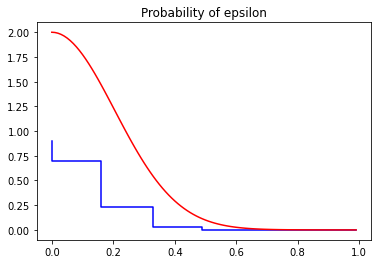
\includegraphics{1.7/1}
        
        The red line is the bound and the blue line is \math{\epsilon}
\end{enumerate}

\section{Problem 1.8}

\begin{enumerate}[a)]
    \item For \math{E(t)}, we have:
        \begin{equation}
            \begin{split}
                E(t) &= \int_{-\infty}^{\infty} t f_t(t)dt \\
                &= \int_{0}^{\infty} t f_t(t)dt \\
                &\geq \int_{\alpha}^{\infty} t f_t(t)dt \\
                &\geq \int_{\alpha}^{\infty} \alpha f_t(t)dt = \alpha \int_{\alpha}^{\infty} f_t(t)dt = \alpha P[t \geq \alpha]
            \end{split}
        \end{equation}
        Thus,
        \begin{equation}
            \begin{split}
                E(t) &\geq \alpha P[t \geq \alpha] \\
                \frac{E(t)}{\alpha} &\geq P[t \geq \alpha]
            \end{split}
        \end{equation}
    \item We know that \math{\sigma^2 = E((u - \mu_u)^2)}. From a), we have:
        \begin{equation}
            \begin{split}
                P[t \geq \alpha] &\leq \frac{E(t)}{\alpha} \text{ , we take u with the equation above} \\
                P[(u - \mu_u)^2 \geq \alpha] &\leq \frac{E((u - \mu_u)^2)}{\alpha} \\
                P[(u - \mu_u)^2 \geq \alpha] &\leq \frac{\sigma^2}{\alpha} \\
            \end{split}
        \end{equation}
    \item From \math{\sigma^2} we have:
        \begin{equation}
            \begin{split}
                \sigma^2 &= Var(u) \\
                &= Var(\frac{1}{N} \sum_{n = 1}^N u_n) \\
                &= \frac{1}{N^2} Var(\sum_{n = 1}^N u_n) \\  % Propriety: Var(cx) = c^2 Var(x) 
                &= \frac{1}{N^2} \sum_{n = 1}^N Var(u_n)  \\ % Propriety
                &= \frac{1}{N^2} N\sigma^2  \\ %
                &= \frac{\sigma^2}{N}
            \end{split}
        \end{equation}
        Combined with the result from b), we have:
        \begin{equation}
            \begin{split}
                P[(u - \mu)^2 \geq \alpha] &\leq \frac{\frac{\sigma^2}{N}}{\alpha} \\
                P[(u - \mu)^2 \geq \alpha] &\leq \frac{\sigma^2}{\Nalpha}
            \end{split}
        \end{equation}
\end{enumerate}

\end{document}
